\documentclass{article}%
\usepackage[T1]{fontenc}%
\usepackage[utf8]{inputenc}%
\usepackage{lmodern}%
\usepackage{textcomp}%
\usepackage{lastpage}%
\usepackage[tmargin=1cm,bmargin=1.5cm,lmargin=1cm,rmargin=1cm]{geometry}%
\usepackage{color}%
\usepackage{ragged2e}%
\usepackage{tikz}%
\usepackage{longtable}%
\usepackage{tabu}%
\usepackage{amsmath}%
\usepackage[table]{xcolor}%
%
\definecolor{cream}{rgb}{0.92 0.92 0.8}%
%
\begin{document}%
\normalsize%
\fontsize{12}{14}%
\selectfont%
\begin{flushleft}%
%
\end{flushleft}%
\section*{Questions: Sinus {-} 3 numbers, 3 digits}%
\label{sec:Questions Sinus {-} 3 numbers, 3 digits}%
Solve questions below:

%
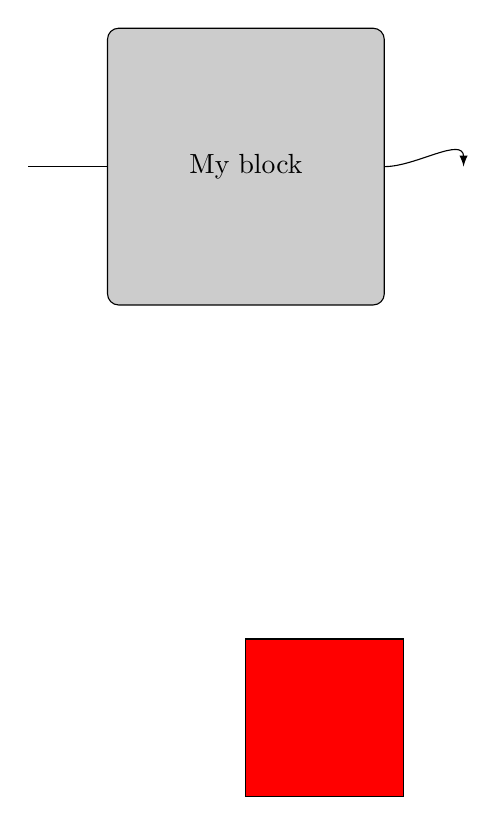
\begin{tikzpicture}%
\node[draw,rounded corners,align=center,minimum size=100pt,fill=black!20] (box) {My block};%
\path[draw,fill=red] (0.0,-6.0) rectangle (2.0,-8.0);%
\path[draw] (box.west) -- ++(-1.0,0.0);%
\path[draw] (box.east) edge[-latex,in=90,out=0] ++(1.0,0.0);%
\end{tikzpicture}%
\renewcommand{\arraystretch}{2.0}%
\begin{longtabu}{X[l] X[l] X[l] }%
\rowcolor{cream}%
\renewcommand{\arraystretch}{1.2}%
\begin{tabular}{ c r }%
\textbf{0:}&$\sin^{2}{\left (x \right )} + \cos^{2}{\left (x \right )}$\\%
\end{tabular}&\renewcommand{\arraystretch}{1.2}%
\begin{tabular}{ c r }%
\textbf{1:}&$\sin^{2}{\left (x \right )} + \cos^{2}{\left (x \right )}$\\%
\end{tabular}&\renewcommand{\arraystretch}{1.2}%
\begin{tabular}{ c r }%
\textbf{2:}&$\sin^{2}{\left (x \right )} + \cos^{2}{\left (x \right )}$\\%
\end{tabular}\\%
\renewcommand{\arraystretch}{1.2}%
\begin{tabular}{ c r }%
\textbf{3:}&$\sin^{2}{\left (x \right )} + \cos^{2}{\left (x \right )}$\\%
\end{tabular}&\renewcommand{\arraystretch}{1.2}%
\begin{tabular}{ c r }%
\textbf{4:}&$\sin^{2}{\left (x \right )} + \cos^{2}{\left (x \right )}$\\%
\end{tabular}&\renewcommand{\arraystretch}{1.2}%
\begin{tabular}{ c r }%
\textbf{5:}&$\sin^{2}{\left (x \right )} + \cos^{2}{\left (x \right )}$\\%
\end{tabular}\\%
\rowcolor{cream}%
\renewcommand{\arraystretch}{1.2}%
\begin{tabular}{ c r }%
\textbf{6:}&$\sin^{2}{\left (x \right )} + \cos^{2}{\left (x \right )}$\\%
\end{tabular}&\renewcommand{\arraystretch}{1.2}%
\begin{tabular}{ c r }%
\textbf{7:}&$\sin^{2}{\left (x \right )} + \cos^{2}{\left (x \right )}$\\%
\end{tabular}&\renewcommand{\arraystretch}{1.2}%
\begin{tabular}{ c r }%
\textbf{8:}&$\sin^{2}{\left (x \right )} + \cos^{2}{\left (x \right )}$\\%
\end{tabular}\\%
\renewcommand{\arraystretch}{1.2}%
\begin{tabular}{ c r }%
\textbf{9:}&$\sin^{2}{\left (x \right )} + \cos^{2}{\left (x \right )}$\\%
\end{tabular}&\renewcommand{\arraystretch}{1.2}%
\begin{tabular}{ c r }%
\textbf{10:}&$\sin^{2}{\left (x \right )} + \cos^{2}{\left (x \right )}$\\%
\end{tabular}&\renewcommand{\arraystretch}{1.2}%
\begin{tabular}{ c r }%
\textbf{11:}&$\sin^{2}{\left (x \right )} + \cos^{2}{\left (x \right )}$\\%
\end{tabular}\\%
\rowcolor{cream}%
\renewcommand{\arraystretch}{1.2}%
\begin{tabular}{ c r }%
\textbf{12:}&$\sin^{2}{\left (x \right )} + \cos^{2}{\left (x \right )}$\\%
\end{tabular}&\renewcommand{\arraystretch}{1.2}%
\begin{tabular}{ c r }%
\textbf{13:}&$\sin^{2}{\left (x \right )} + \cos^{2}{\left (x \right )}$\\%
\end{tabular}&\renewcommand{\arraystretch}{1.2}%
\begin{tabular}{ c r }%
\textbf{14:}&$\sin^{2}{\left (x \right )} + \cos^{2}{\left (x \right )}$\\%
\end{tabular}\\%
\renewcommand{\arraystretch}{1.2}%
\begin{tabular}{ c r }%
\textbf{15:}&$\sin^{2}{\left (x \right )} + \cos^{2}{\left (x \right )}$\\%
\end{tabular}&\renewcommand{\arraystretch}{1.2}%
\begin{tabular}{ c r }%
\textbf{16:}&$\sin^{2}{\left (x \right )} + \cos^{2}{\left (x \right )}$\\%
\end{tabular}&\renewcommand{\arraystretch}{1.2}%
\begin{tabular}{ c r }%
\textbf{17:}&$\sin^{2}{\left (x \right )} + \cos^{2}{\left (x \right )}$\\%
\end{tabular}\\%
\rowcolor{cream}%
\renewcommand{\arraystretch}{1.2}%
\begin{tabular}{ c r }%
\textbf{18:}&$\sin^{2}{\left (x \right )} + \cos^{2}{\left (x \right )}$\\%
\end{tabular}&\renewcommand{\arraystretch}{1.2}%
\begin{tabular}{ c r }%
\textbf{19:}&$\sin^{2}{\left (x \right )} + \cos^{2}{\left (x \right )}$\\%
\end{tabular}&\renewcommand{\arraystretch}{1.2}%
\begin{tabular}{ c r }%
\textbf{20:}&$\sin^{2}{\left (x \right )} + \cos^{2}{\left (x \right )}$\\%
\end{tabular}\\%
\renewcommand{\arraystretch}{1.2}%
\begin{tabular}{ c r }%
\textbf{21:}&$\sin^{2}{\left (x \right )} + \cos^{2}{\left (x \right )}$\\%
\end{tabular}&\renewcommand{\arraystretch}{1.2}%
\begin{tabular}{ c r }%
\textbf{22:}&$\sin^{2}{\left (x \right )} + \cos^{2}{\left (x \right )}$\\%
\end{tabular}&\renewcommand{\arraystretch}{1.2}%
\begin{tabular}{ c r }%
\textbf{23:}&$\sin^{2}{\left (x \right )} + \cos^{2}{\left (x \right )}$\\%
\end{tabular}\\%
\rowcolor{cream}%
\renewcommand{\arraystretch}{1.2}%
\begin{tabular}{ c r }%
\textbf{24:}&$\sin^{2}{\left (x \right )} + \cos^{2}{\left (x \right )}$\\%
\end{tabular}&\renewcommand{\arraystretch}{1.2}%
\begin{tabular}{ c r }%
\textbf{25:}&$\sin^{2}{\left (x \right )} + \cos^{2}{\left (x \right )}$\\%
\end{tabular}&\renewcommand{\arraystretch}{1.2}%
\begin{tabular}{ c r }%
\textbf{26:}&$\sin^{2}{\left (x \right )} + \cos^{2}{\left (x \right )}$\\%
\end{tabular}\\%
\renewcommand{\arraystretch}{1.2}%
\begin{tabular}{ c r }%
\textbf{27:}&$\sin^{2}{\left (x \right )} + \cos^{2}{\left (x \right )}$\\%
\end{tabular}&\renewcommand{\arraystretch}{1.2}%
\begin{tabular}{ c r }%
\textbf{28:}&$\sin^{2}{\left (x \right )} + \cos^{2}{\left (x \right )}$\\%
\end{tabular}&\renewcommand{\arraystretch}{1.2}%
\begin{tabular}{ c r }%
\textbf{29:}&$\sin^{2}{\left (x \right )} + \cos^{2}{\left (x \right )}$\\%
\end{tabular}\\%
\rowcolor{cream}%
\renewcommand{\arraystretch}{1.2}%
\begin{tabular}{ c r }%
\textbf{30:}&$\sin^{2}{\left (x \right )} + \cos^{2}{\left (x \right )}$\\%
\end{tabular}&\renewcommand{\arraystretch}{1.2}%
\begin{tabular}{ c r }%
\textbf{31:}&$\sin^{2}{\left (x \right )} + \cos^{2}{\left (x \right )}$\\%
\end{tabular}&\renewcommand{\arraystretch}{1.2}%
\begin{tabular}{ c r }%
\textbf{32:}&$\sin^{2}{\left (x \right )} + \cos^{2}{\left (x \right )}$\\%
\end{tabular}\\%
\renewcommand{\arraystretch}{1.2}%
\begin{tabular}{ c r }%
\textbf{33:}&$\sin^{2}{\left (x \right )} + \cos^{2}{\left (x \right )}$\\%
\end{tabular}&\renewcommand{\arraystretch}{1.2}%
\begin{tabular}{ c r }%
\textbf{34:}&$\sin^{2}{\left (x \right )} + \cos^{2}{\left (x \right )}$\\%
\end{tabular}&\renewcommand{\arraystretch}{1.2}%
\begin{tabular}{ c r }%
\textbf{35:}&$\sin^{2}{\left (x \right )} + \cos^{2}{\left (x \right )}$\\%
\end{tabular}\\%
\rowcolor{cream}%
\renewcommand{\arraystretch}{1.2}%
\begin{tabular}{ c r }%
\textbf{36:}&$\sin^{2}{\left (x \right )} + \cos^{2}{\left (x \right )}$\\%
\end{tabular}&\renewcommand{\arraystretch}{1.2}%
\begin{tabular}{ c r }%
\textbf{37:}&$\sin^{2}{\left (x \right )} + \cos^{2}{\left (x \right )}$\\%
\end{tabular}&\renewcommand{\arraystretch}{1.2}%
\begin{tabular}{ c r }%
\textbf{38:}&$\sin^{2}{\left (x \right )} + \cos^{2}{\left (x \right )}$\\%
\end{tabular}\\%
\renewcommand{\arraystretch}{1.2}%
\begin{tabular}{ c r }%
\textbf{39:}&$\sin^{2}{\left (x \right )} + \cos^{2}{\left (x \right )}$\\%
\end{tabular}&\renewcommand{\arraystretch}{1.2}%
\begin{tabular}{ c r }%
\textbf{40:}&$\sin^{2}{\left (x \right )} + \cos^{2}{\left (x \right )}$\\%
\end{tabular}&\renewcommand{\arraystretch}{1.2}%
\begin{tabular}{ c r }%
\textbf{41:}&$\sin^{2}{\left (x \right )} + \cos^{2}{\left (x \right )}$\\%
\end{tabular}\\%
\rowcolor{cream}%
\renewcommand{\arraystretch}{1.2}%
\begin{tabular}{ c r }%
\textbf{42:}&$\sin^{2}{\left (x \right )} + \cos^{2}{\left (x \right )}$\\%
\end{tabular}&\renewcommand{\arraystretch}{1.2}%
\begin{tabular}{ c r }%
\textbf{43:}&$\sin^{2}{\left (x \right )} + \cos^{2}{\left (x \right )}$\\%
\end{tabular}&\renewcommand{\arraystretch}{1.2}%
\begin{tabular}{ c r }%
\textbf{44:}&$\sin^{2}{\left (x \right )} + \cos^{2}{\left (x \right )}$\\%
\end{tabular}\\%
\renewcommand{\arraystretch}{1.2}%
\begin{tabular}{ c r }%
\textbf{45:}&$\sin^{2}{\left (x \right )} + \cos^{2}{\left (x \right )}$\\%
\end{tabular}&\renewcommand{\arraystretch}{1.2}%
\begin{tabular}{ c r }%
\textbf{46:}&$\sin^{2}{\left (x \right )} + \cos^{2}{\left (x \right )}$\\%
\end{tabular}&\renewcommand{\arraystretch}{1.2}%
\begin{tabular}{ c r }%
\textbf{47:}&$\sin^{2}{\left (x \right )} + \cos^{2}{\left (x \right )}$\\%
\end{tabular}\\%
\rowcolor{cream}%
\renewcommand{\arraystretch}{1.2}%
\begin{tabular}{ c r }%
\textbf{48:}&$\sin^{2}{\left (x \right )} + \cos^{2}{\left (x \right )}$\\%
\end{tabular}&\renewcommand{\arraystretch}{1.2}%
\begin{tabular}{ c r }%
\textbf{49:}&$\sin^{2}{\left (x \right )} + \cos^{2}{\left (x \right )}$\\%
\end{tabular}&\renewcommand{\arraystretch}{1.2}%
\begin{tabular}{ c r }%
\textbf{50:}&$\sin^{2}{\left (x \right )} + \cos^{2}{\left (x \right )}$\\%
\end{tabular}\\%
\renewcommand{\arraystretch}{1.2}%
\begin{tabular}{ c r }%
\textbf{51:}&$\sin^{2}{\left (x \right )} + \cos^{2}{\left (x \right )}$\\%
\end{tabular}&\renewcommand{\arraystretch}{1.2}%
\begin{tabular}{ c r }%
\textbf{52:}&$\sin^{2}{\left (x \right )} + \cos^{2}{\left (x \right )}$\\%
\end{tabular}&\renewcommand{\arraystretch}{1.2}%
\begin{tabular}{ c r }%
\textbf{53:}&$\sin^{2}{\left (x \right )} + \cos^{2}{\left (x \right )}$\\%
\end{tabular}\\%
\rowcolor{cream}%
\renewcommand{\arraystretch}{1.2}%
\begin{tabular}{ c r }%
\textbf{54:}&$\sin^{2}{\left (x \right )} + \cos^{2}{\left (x \right )}$\\%
\end{tabular}&\renewcommand{\arraystretch}{1.2}%
\begin{tabular}{ c r }%
\textbf{55:}&$\sin^{2}{\left (x \right )} + \cos^{2}{\left (x \right )}$\\%
\end{tabular}&\renewcommand{\arraystretch}{1.2}%
\begin{tabular}{ c r }%
\textbf{56:}&$\sin^{2}{\left (x \right )} + \cos^{2}{\left (x \right )}$\\%
\end{tabular}\\%
\renewcommand{\arraystretch}{1.2}%
\begin{tabular}{ c r }%
\textbf{57:}&$\sin^{2}{\left (x \right )} + \cos^{2}{\left (x \right )}$\\%
\end{tabular}&\renewcommand{\arraystretch}{1.2}%
\begin{tabular}{ c r }%
\textbf{58:}&$\sin^{2}{\left (x \right )} + \cos^{2}{\left (x \right )}$\\%
\end{tabular}&\renewcommand{\arraystretch}{1.2}%
\begin{tabular}{ c r }%
\textbf{59:}&$\sin^{2}{\left (x \right )} + \cos^{2}{\left (x \right )}$\\%
\end{tabular}\\%
\rowcolor{cream}%
\renewcommand{\arraystretch}{1.2}%
\begin{tabular}{ c r }%
\textbf{60:}&$\sin^{2}{\left (x \right )} + \cos^{2}{\left (x \right )}$\\%
\end{tabular}&\renewcommand{\arraystretch}{1.2}%
\begin{tabular}{ c r }%
\textbf{61:}&$\sin^{2}{\left (x \right )} + \cos^{2}{\left (x \right )}$\\%
\end{tabular}&\renewcommand{\arraystretch}{1.2}%
\begin{tabular}{ c r }%
\textbf{62:}&$\sin^{2}{\left (x \right )} + \cos^{2}{\left (x \right )}$\\%
\end{tabular}\\%
\renewcommand{\arraystretch}{1.2}%
\begin{tabular}{ c r }%
\textbf{63:}&$\sin^{2}{\left (x \right )} + \cos^{2}{\left (x \right )}$\\%
\end{tabular}&\renewcommand{\arraystretch}{1.2}%
\begin{tabular}{ c r }%
\textbf{64:}&$\sin^{2}{\left (x \right )} + \cos^{2}{\left (x \right )}$\\%
\end{tabular}&\renewcommand{\arraystretch}{1.2}%
\begin{tabular}{ c r }%
\textbf{65:}&$\sin^{2}{\left (x \right )} + \cos^{2}{\left (x \right )}$\\%
\end{tabular}\\%
\rowcolor{cream}%
\renewcommand{\arraystretch}{1.2}%
\begin{tabular}{ c r }%
\textbf{66:}&$\sin^{2}{\left (x \right )} + \cos^{2}{\left (x \right )}$\\%
\end{tabular}&\renewcommand{\arraystretch}{1.2}%
\begin{tabular}{ c r }%
\textbf{67:}&$\sin^{2}{\left (x \right )} + \cos^{2}{\left (x \right )}$\\%
\end{tabular}&\renewcommand{\arraystretch}{1.2}%
\begin{tabular}{ c r }%
\textbf{68:}&$\sin^{2}{\left (x \right )} + \cos^{2}{\left (x \right )}$\\%
\end{tabular}\\%
\renewcommand{\arraystretch}{1.2}%
\begin{tabular}{ c r }%
\textbf{69:}&$\sin^{2}{\left (x \right )} + \cos^{2}{\left (x \right )}$\\%
\end{tabular}&\renewcommand{\arraystretch}{1.2}%
\begin{tabular}{ c r }%
\textbf{70:}&$\sin^{2}{\left (x \right )} + \cos^{2}{\left (x \right )}$\\%
\end{tabular}&\renewcommand{\arraystretch}{1.2}%
\begin{tabular}{ c r }%
\textbf{71:}&$\sin^{2}{\left (x \right )} + \cos^{2}{\left (x \right )}$\\%
\end{tabular}\\%
\rowcolor{cream}%
\renewcommand{\arraystretch}{1.2}%
\begin{tabular}{ c r }%
\textbf{72:}&$\sin^{2}{\left (x \right )} + \cos^{2}{\left (x \right )}$\\%
\end{tabular}&\renewcommand{\arraystretch}{1.2}%
\begin{tabular}{ c r }%
\textbf{73:}&$\sin^{2}{\left (x \right )} + \cos^{2}{\left (x \right )}$\\%
\end{tabular}&\renewcommand{\arraystretch}{1.2}%
\begin{tabular}{ c r }%
\textbf{74:}&$\sin^{2}{\left (x \right )} + \cos^{2}{\left (x \right )}$\\%
\end{tabular}\\%
\renewcommand{\arraystretch}{1.2}%
\begin{tabular}{ c r }%
\textbf{75:}&$\sin^{2}{\left (x \right )} + \cos^{2}{\left (x \right )}$\\%
\end{tabular}&\renewcommand{\arraystretch}{1.2}%
\begin{tabular}{ c r }%
\textbf{76:}&$\sin^{2}{\left (x \right )} + \cos^{2}{\left (x \right )}$\\%
\end{tabular}&\renewcommand{\arraystretch}{1.2}%
\begin{tabular}{ c r }%
\textbf{77:}&$\sin^{2}{\left (x \right )} + \cos^{2}{\left (x \right )}$\\%
\end{tabular}\\%
\rowcolor{cream}%
\renewcommand{\arraystretch}{1.2}%
\begin{tabular}{ c r }%
\textbf{78:}&$\sin^{2}{\left (x \right )} + \cos^{2}{\left (x \right )}$\\%
\end{tabular}&\renewcommand{\arraystretch}{1.2}%
\begin{tabular}{ c r }%
\textbf{79:}&$\sin^{2}{\left (x \right )} + \cos^{2}{\left (x \right )}$\\%
\end{tabular}&\renewcommand{\arraystretch}{1.2}%
\begin{tabular}{ c r }%
\textbf{80:}&$\sin^{2}{\left (x \right )} + \cos^{2}{\left (x \right )}$\\%
\end{tabular}\\%
\renewcommand{\arraystretch}{1.2}%
\begin{tabular}{ c r }%
\textbf{81:}&$\sin^{2}{\left (x \right )} + \cos^{2}{\left (x \right )}$\\%
\end{tabular}&\renewcommand{\arraystretch}{1.2}%
\begin{tabular}{ c r }%
\textbf{82:}&$\sin^{2}{\left (x \right )} + \cos^{2}{\left (x \right )}$\\%
\end{tabular}&\renewcommand{\arraystretch}{1.2}%
\begin{tabular}{ c r }%
\textbf{83:}&$\sin^{2}{\left (x \right )} + \cos^{2}{\left (x \right )}$\\%
\end{tabular}\\%
\rowcolor{cream}%
\renewcommand{\arraystretch}{1.2}%
\begin{tabular}{ c r }%
\textbf{84:}&$\sin^{2}{\left (x \right )} + \cos^{2}{\left (x \right )}$\\%
\end{tabular}&\renewcommand{\arraystretch}{1.2}%
\begin{tabular}{ c r }%
\textbf{85:}&$\sin^{2}{\left (x \right )} + \cos^{2}{\left (x \right )}$\\%
\end{tabular}&\renewcommand{\arraystretch}{1.2}%
\begin{tabular}{ c r }%
\textbf{86:}&$\sin^{2}{\left (x \right )} + \cos^{2}{\left (x \right )}$\\%
\end{tabular}\\%
\renewcommand{\arraystretch}{1.2}%
\begin{tabular}{ c r }%
\textbf{87:}&$\sin^{2}{\left (x \right )} + \cos^{2}{\left (x \right )}$\\%
\end{tabular}&\renewcommand{\arraystretch}{1.2}%
\begin{tabular}{ c r }%
\textbf{88:}&$\sin^{2}{\left (x \right )} + \cos^{2}{\left (x \right )}$\\%
\end{tabular}&\renewcommand{\arraystretch}{1.2}%
\begin{tabular}{ c r }%
\textbf{89:}&$\sin^{2}{\left (x \right )} + \cos^{2}{\left (x \right )}$\\%
\end{tabular}\\%
\rowcolor{cream}%
\renewcommand{\arraystretch}{1.2}%
\begin{tabular}{ c r }%
\textbf{90:}&$\sin^{2}{\left (x \right )} + \cos^{2}{\left (x \right )}$\\%
\end{tabular}&\renewcommand{\arraystretch}{1.2}%
\begin{tabular}{ c r }%
\textbf{91:}&$\sin^{2}{\left (x \right )} + \cos^{2}{\left (x \right )}$\\%
\end{tabular}&\renewcommand{\arraystretch}{1.2}%
\begin{tabular}{ c r }%
\textbf{92:}&$\sin^{2}{\left (x \right )} + \cos^{2}{\left (x \right )}$\\%
\end{tabular}\\%
\renewcommand{\arraystretch}{1.2}%
\begin{tabular}{ c r }%
\textbf{93:}&$\sin^{2}{\left (x \right )} + \cos^{2}{\left (x \right )}$\\%
\end{tabular}&\renewcommand{\arraystretch}{1.2}%
\begin{tabular}{ c r }%
\textbf{94:}&$\sin^{2}{\left (x \right )} + \cos^{2}{\left (x \right )}$\\%
\end{tabular}&\renewcommand{\arraystretch}{1.2}%
\begin{tabular}{ c r }%
\textbf{95:}&$\sin^{2}{\left (x \right )} + \cos^{2}{\left (x \right )}$\\%
\end{tabular}\\%
\rowcolor{cream}%
\renewcommand{\arraystretch}{1.2}%
\begin{tabular}{ c r }%
\textbf{96:}&$\sin^{2}{\left (x \right )} + \cos^{2}{\left (x \right )}$\\%
\end{tabular}&\renewcommand{\arraystretch}{1.2}%
\begin{tabular}{ c r }%
\textbf{97:}&$\sin^{2}{\left (x \right )} + \cos^{2}{\left (x \right )}$\\%
\end{tabular}&\renewcommand{\arraystretch}{1.2}%
\begin{tabular}{ c r }%
\textbf{98:}&$\sin^{2}{\left (x \right )} + \cos^{2}{\left (x \right )}$\\%
\end{tabular}\\%
\renewcommand{\arraystretch}{1.2}%
\begin{tabular}{ c r }%
\textbf{99:}&$\sin^{2}{\left (x \right )} + \cos^{2}{\left (x \right )}$\\%
\end{tabular}&\renewcommand{\arraystretch}{1.2}%
\begin{tabular}{ c r }%
\textbf{100:}&$\sin^{2}{\left (x \right )} + \cos^{2}{\left (x \right )}$\\%
\end{tabular}&\renewcommand{\arraystretch}{1.2}%
\begin{tabular}{ c r }%
\textbf{101:}&$\sin^{2}{\left (x \right )} + \cos^{2}{\left (x \right )}$\\%
\end{tabular}\\%
\end{longtabu}%
\end{document}